\documentclass[10pt, a4paper]{article}
\usepackage[utf8]{inputenc}
\usepackage[UKenglish]{babel}
% \usepackage{fontspec}
\usepackage{xcolor, graphicx}
\usepackage{makeidx}
\usepackage[scale=0.85]{sourcecodepro}
\usepackage{amsmath, amssymb, amsfonts}
\usepackage{microtype}
\usepackage{comment}
\usepackage{physics}
\usepackage{siunitx}
\usepackage{tikz}
\usepackage{bookmark}
\usepackage{geometry}

\usepackage[print=m, lang=fortran, verbose]{fortex}

\makeindex

\usetikzlibrary{decorations.markings}
\definecolor{fortexbg}{HTML}{F8F8F0}
\definecolor{fortextab}{HTML}{C0C0A8}
\usemintedstyle{ayu}
\setfortex{tabsize=2, breaksymbol=\scriptsize{$\hookrightarrow$}, fontsize=\small, breaklines, bgcolor=fortexbg, showtabs, tab={\rm{$\big|\hspace{0.825ex}$}}, tabcolor={fortextab}}
\DefineShortVerb{\"}

\begin{document}

\section{Introduction}

The aim of this module is to provide a \emph{fake} monopole. Not one generated by simulation, but by looking at monopoles that are generated by simulation, and then trying to match feature for feature. 
The reason all this exists is that I want to train a neural network to detect monopoles in the RICH1 data, but generating monopoles takes half and hour each. 

So in order to get the large datasets needed to train the NN, I am generating fake data. 
The aim is to make it as accurate as possible to the real dataset, but it remains to be seen how that goes. 

The simulated monopoles have been generated by Bender and LOKI. Note that I am trying to match a simulation and that simulation may be incorrect. This is to be expected, but what can you do? no-one has ever seen a monopole. 

\begin{code}
module nn_fake_gendata
	use ISO_C_BINDING
	use stdlib_math, only: arange
	use stdlib_stats_distribution_normal, only: rvs_normal 
	use stdlib_stats_distribution_uniform, only: shuffle, rvs_uniform
	use stdlib_stats_distribution_exponential, only: rvs_exp
	use writeimgf
	
	implicit none
	
	private 
	public :: mk_griddata
	
	real :: M_2PI
	parameter( M_2PI = 8. * ATAN(1.) )
\end{code}

Here $A_s \times A_s$ is the sensor area. Each detector has area $1302 \times 555$ \si{\milli \metre}

\begin{codevar}{A_s}
\begin{code}
	real :: A_s(2)
	parameter( A_s = [ 1302., 555.* 2.])
\end{code}
\end{codevar}

And $A_i \times A_i$ is the dimensions of the output image that is going to be generated. Here I am normalising the first $1302$ \si{\milli \metre} axis to have $128$ pixels, thus the $555$ \si{\milli \metre} axis has $109$ pixels.

We also note that FFTW3 does not work very well for images that are not powers of 2. This is evidences by the computation times going from $27$ \si{\second} to $8.5$ \si{\second} when the image size is \emph{increased} from $128 \times 109$ to $128 \times 128$.

As such we define a padded image $A_p$ that is greater or equal to the actual inage dimensions we are interested in.

\begin{codevar}{A_i, A_p, sensor_basis_1, sensor_basis_2, sensor_gap, sensor_radi, sensor_stamp}
\begin{code}
	integer :: A_i(2)
	parameter( A_i = nint(A_s * 128. / 1302.) )
	integer :: A_p
	parameter( A_p = 128 )
	
	real    :: sensor_basis_1(2), sensor_basis_2(2), sensor_gap, sensor_radi
	parameter( sensor_gap     = 0.8 ,                                            &
	           sensor_radi    = 4.  ,                                            &
	           sensor_basis_1 = [ 2. * sensor_radi, 0. ] + [ sensor_gap, 0. ] ,  &
	           sensor_basis_2 = [ sensor_radi, sqrt(3.) * sensor_radi ] +        & 
	                            [ 1./2. * sensor_gap, sqrt(3.)/2. * sensor_gap ] &
	)
	logical :: sensor_stamp(-nint(sensor_radi):nint(sensor_radi),  & 
	                        -nint(sensor_radi):nint(sensor_radi) )
	
contains 
\end{code}
\end{codevar}

\clearpage
\section{Sensor Grid}

One of the problem that has to be dealt with is that the sensor does not cover the entire plane, but is rather divided into circles 

\begin{figure}[h]
\centering 
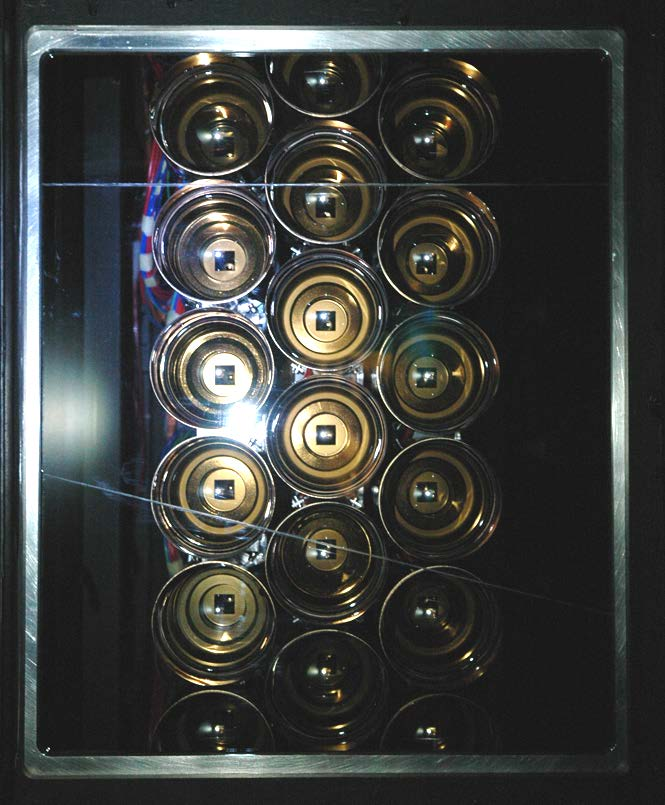
\includegraphics[width=0.3\textwidth]{Images/photocathode.png}
\caption{The photocathodes of RICH1}
\end{figure}

We need to emulate this grid for our fake data. 
At the moment I don't have a good reference for how the grid is actually laid out so for now I am going to pretend that it is a hexagonal grid over the whole area (even though I know that the sensing area is divided into two. 

To deal with this The idea is to create a mask that we can then use to filter against using Fortran's "pack" intrinsic.

here $r$ is the radius of each sensor and $g$ is the gap size between the sensors.

\begin{codeblock}{sensor}
\begin{code}
function sensor() result(retval)
	logical, dimension(A_p, A_p) :: retval
	
	integer :: s_s 
	real :: p(2)
	integer :: p_i(2)
	integer :: x, y
	
	s_s = ceiling(sensor_radi)
\end{code}

Here we are defining the basis vectors $e_1$ and $e_2$. the aim is to step along $e_1$ stamping a circle at each step. 
Then once we hit the right hand edge, we increment by $e_2$, then unwind $e_1$ back to the left of the image. 

\begin{figure}[h!]
\centering
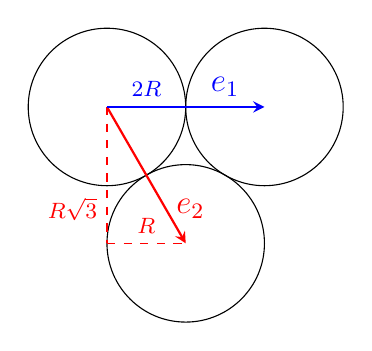
\begin{tikzpicture}[>=stealth]
	\draw (0, 0) circle [radius = 1];
	\draw (2, 0) circle [radius = 1];
	\draw (1, -1.732) circle [radius = 1];
	\draw[red, dashed] (0, -1.732) -- (1, -1.732) node [midway, above] {\footnotesize$R$};
	\draw[red, dashed] (0, 0) -- (0, -1.732) node [near end, left] {\footnotesize$R\sqrt{3}$};
	\draw[thick, red, ->] (0, 0) -- (1, -1.732) node [near end, right]{\large$e_2$};
	\draw[thick, blue, ->] (0, 0) -- (2, 0) node [near end, above]{\large$e_1$} node [near start, above] {\footnotesize$2R$};
\end{tikzpicture}
\end{figure}

Here $p$ is the current location of the stamp, and $p_i$ is the integer version used for indexing
\begin{code}
	p = [sensor_radi, sensor_radi]
\end{code}

The stamp itself if just a circle, with radii $r$, contained in a zero-centred array of the same size.

\begin{code}
	sensor_stamp = .False.
	do concurrent (x = -s_s:s_s, y= -s_s:s_s)
		if ( x**2 + y**2 < sensor_radi**2 ) then 
			sensor_stamp(x, y) = .True.
		end if 
	end do
\end{code}

This indexing looks complex, but its not too bad. Here we are just slicing "retval" to be the same size as "stamp". with the centre position of the slice given by $p$.

Note that we have to use ".or." here, otherwise the corners of the stamp (where all the ".False." live), will overlap on the previously defined circle.


\begin{code}
	retval = .False.
	
	do while ( p(2) < A_i(2) - s_s - 1 )
		p_i = nint( p + 1 )
		
		associate( retval => retval( p_i(1)-s_s : p_i(1)+s_s , p_i(2)-s_s : p_i(2)+s_s ) )
			retval = retval .or. sensor_stamp
		end associate 
			
\end{code}

Here is where the unrolling logic lives. The main thing to be careful of here is that you need to define the "do while" loop to be one basis vector shorter than the edge of the array. 

\begin{figure}[h]
\centering
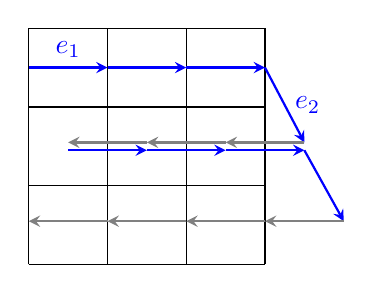
\begin{tikzpicture}[>=stealth]
	\draw[step=1] (0,0) grid (3,-3);
	\draw[blue, ->, thick] (0, -0.5) -> ++(1, 0) node[midway, above] {$e_1$};
	\foreach \x in {1, ..., 2} {
		\draw[blue, ->, thick] (\x, -0.5)-> ++(1, 0);
	}
	\draw[blue, ->, thick] (3, -0.5) -> (3 + 0.5, -1.45) node[midway, right] {$e_2$};
	\foreach \x in {3, ..., 1} {
		\draw[gray, ->, thick] (\x +0.5, -1.45) -> ++(-1, 0);
		\draw[blue, ->, thick] (\x -0.5, -1.55) -> ++(1, 0);
	}
	\draw[blue, ->, thick] (3+0.5, -1.55) -> (4, -2.45);
	\foreach \x in {4, ..., 1} {
		\draw[gray, ->, thick] (\x, -2.45) -> ++(-1, 0);
	}
\end{tikzpicture}
\caption{Stamping happens every time the offset vector $p$ is still inside the image. Here the unwinding of $e_1$ is represented in grey.}
\end{figure}

\begin{code}
		p = p + sensor_basis_1
		if ( p(1) > A_i(1) - sensor_radi) then 
			p = p + sensor_basis_2 
			do while ( p(1) > sensor_basis_1(1) + 1  )
				p = p - sensor_basis_1
			end do 
		end if 
		
	end do 
end function
\end{code}
\end{codeblock}
 
\section{Faux Data Generation}

\subsection{Background Only}

Here we are creating the situation where there is no monopole in the data. 

By fitting it was found that the number of hits per event was an exponential distribution with $\lambda = 1.11 \cdot 10^{-3}$. 

From here we distribute the hits randomly over the detector. 

The real detector is divided up into discrete pixels and these pixels are packed into circular sensing regions. 
At the moment I am not simulating this as I just cannot be bothered. 

\begin{codeblock}{background}
\begin{code}
subroutine background(x, y, N)
	integer, intent(out) :: N
	real, intent(out), allocatable :: x(:), y(:)
	complex, allocatable :: c(:)
	logical, allocatable :: m(:)
	
	complex, allocatable :: p(:, :)
	logical, allocatable :: m_p(:, :)
	integer, allocatable :: N_p
	
	integer :: i 
	real :: r(20)
	
	n_z: do while (.True.)
		N = int(rvs_exp(1.11E-3))
		if (N /= 0) then 
			exit n_z 
		end if
	end do n_z
	
	call extra_bg(1000., 100., cmplx(0, 0), 100., c, m)
	
	call random_number(r)
	N_p = count(r > 0.5)+1
	
	allocate( p(N_p, 10),  m_p(N_p, 10) )

	do i = 1, N_p
		p(i, :) = rvs_normal( cmplx(A_s(2)*rand(0)-A_s(2)/2.,  &
		                            A_s(1)*rand(0)-A_s(1)/2.), &
		                      cmplx(10., 10.),                 &
		                      10)
	end do
	m_p = ( abs(real(p)) < A_s(2)/2. ) .and. ( abs(aimag(p)) < A_s(1)/2. )
	
	
	allocate( x(N + count(m) + count(m_p)), y(N + count(m) + count(m_p)) )
	
	x = [rvs_uniform(-A_s(2)/2., A_s(2), N ), pack( real(c), m), pack( real(p), m_p)]
	y = [rvs_uniform(-A_s(1)/2., A_s(1), N ), pack(aimag(c), m), pack(aimag(p), m_p)]
	
	N = N + count(m) + count(m_p)
end subroutine
\end{code}
\end{codeblock}

\subsection{Monopole and background}

For the positive detections, we superimpose a monopole event on the background events.

To create the monopole ring that we aim to detect we are using the fact that $e^{i\theta}$ is a circle for $\theta \in [0, 2\pi)$. from there we can scale and displace this circle, and take the real and imaginary components as the $(x,y)$ coordinates.

Note that we multiply the radius by a normal distribution to make sure it is not a perfect circle, but rather a bit of a fuzzy one.
Note also that due to the detectors living in a $x, y \in [-600, 600]$ square, we need to make sure to prune any detections of the monopole that happen outside this range.

though tout this function variables ending in "_a" relate to the aerogel, and "_g" the gas. Furthermore, "_bg" refers to events that are not generated by the monopole itself, but rather the background.  

\begin{codeblock}{monopole}
\begin{code}
subroutine monopole(x, y, N, eta, beta)
	real, intent(out), allocatable :: x(:), y(:)
	real, intent(out) :: eta, beta
	integer, intent(out) :: N 
	
	real, allocatable :: x_bg(:), y_bg(:)
	integer :: N_bg 
	
	integer :: N_a, N_g
	real    :: R_a, R_g
	complex, allocatable :: c_a(:), c_g(:)
	logical, allocatable :: m_a(:), m_g(:)
	real   , allocatable :: theta_a(:), theta_g(:)
	
	complex, allocatable :: c_extra_bg(:)
	logical, allocatable :: m_extra_bg(:)
	
	integer, allocatable :: shuf_i(:)	
\end{code}

As we have 2 circles from the monopole (one from the aerogel and one from the $\text{C}_4 \text{F}_10$), we save where the monopole is centred so we can use it as an offset. 

As our sensor has bounds $x, y \in [-600, 600]$, we set the centre of the monopole to be in this range. 

In the future I mught figure out how much monopole needs to be outside these bounds. 

\begin{code}
	complex :: p 
	eta = 0
	p = rvs_uniform(cmplx(-A_s(2)/2. , -A_s(1)/2.), cmplx(A_s(2), A_s(1)))
	eta = mono_eta(p)
\end{code}

Assuming that the background rate is not affected by the presence of a monopole. 
I know this is a false assumption as the background higher in the presence of a monopole (looks kinda Gaussian). 
But for the moment this is a good enough assumption.

\begin{code}
	call background(x_bg, y_bg, N_bg)
\end{code}

Our code has the (\emph{very} small) chance that it will choose a monopole so heavy and slow that no Cherenkov appears. 
Physically this is totally possible to happen, but for out usecase, this is basically pointless as we don't care about monopoles tat we cannot see or detect. 

As such we make sure that if a monopole is going to appear in the image, that a monopole actually appears. 

\begin{code}
	ck_mono: do while (.True.)
		beta = 0
		call mono_beta(1.03,   0.16, N_a, R_a, beta)
		call mono_beta(1.0014, 1.  , N_g, R_g, beta)
		
		if ( (N_a > 0) .or. (N_g > 0) ) then 
			exit ck_mono
		end if
	end do ck_mono
	
	allocate(theta_a(N_a), c_a(N_a), m_a(N_a))
	allocate(theta_g(N_g), c_g(N_g), m_g(N_g))
	
	call random_number(theta_a)
	call random_number(theta_g)
\end{code}

Here we are using complex numbers to generate the circle. Theoretically this could be done separately with both $x$, and $y$ separately, but this makes the maths neater. 

Here the circle sizes and standard deviations have been measured from the simulation data. 
the radii $R_\text{aero} = 375\pm11$ and $R_\text{CF} = 75 \pm 21$. 

Note that these are a little bit larger than the ones measured off the graph.


We are also broadening the radii to match that of the graph, however I am doing this with values measured off the graph.

\begin{code}
	c_a = rvs_normal(R_a, 11. , N_a ) * exp(cmplx(0, M_2PI * theta_a )) - p
	c_g = rvs_normal(R_g, 21. , N_g ) * exp(cmplx(0, M_2PI * theta_g )) - p
\end{code}

As the centre of the circle appears anywhere inside the sensor, the circle itself by definition will have sections outside the sensor (as far out as 1 radius). 
As such we will not see those and so we prune the output to only those pixels inside the sensor region 

\begin{code}
	deallocate(theta_a, theta_g)
	
	m_a = abs(real(c_a)) < A_s(2)/2. .and. abs(aimag(c_a)) < A_s(1)/2.
	m_g = abs(real(c_g)) < A_s(2)/2. .and. abs(aimag(c_g)) < A_s(1)/2.
\end{code}

\begin{code}
	call extra_bg(500., 500., p, R_a, c_extra_bg, m_extra_bg)
\end{code}

\begin{code}
	N = N_bg + count(m_a) + count(m_g) + count(m_extra_bg)
	
	allocate(x(N), y(N), shuf_i(N))
	
	x = [x_bg, pack(real(c_g),  m_g),  pack(real(c_a),  m_a), pack(real(c_extra_bg) , m_extra_bg)]
	y = [y_bg, pack(aimag(c_g), m_g),  pack(aimag(c_a), m_a), pack(aimag(c_extra_bg), m_extra_bg)]
	
	deallocate(x_bg, y_bg, c_a, c_g, m_a, m_g, c_extra_bg, m_extra_bg)
\end{code}

The data should not come in ordered. This doesn't matter if we are placing it all onto a grid, but for a NN that does not use pictures, but rather raw sets of $x$,$y$ data, this is important. 

\begin{code}
	shuf_i = shuffle(arange(N))
	x = x(shuf_i)
	y = y(shuf_i)
	
	deallocate(shuf_i)
end subroutine
\end{code}
\end{codeblock}

One thing that we might want to consider is how fast the monopole is moving. 
As the condition for Cherenkov radiation is:

\begin{equation}
\frac{1}{n} < \beta
\end{equation}

and the angle of emission is defined as:

\begin{equation}
\cos(\theta) = \frac{1}{n\beta}
\end{equation}

This shows that both the number of rings and the size of the rings depend on how fast the monopole is travelling. 
As we at the moment have no idea what mass the monopole is, we hence have no idea how fast the monopole is travelling. 

finally the number of photons emitted by the monopole;

\begin{equation}
 \frac{\dd^2 n_\gamma}{\dd \ell \dd \lambda} = \frac{2 \pi \alpha}{\lambda ^2} \left( \frac{gn}{e}\right)^2\left( 1 - \frac{1}{\beta^2_\text{m}n^2}\right) \label{eqn:ng}
\end{equation}

One thing to note however is that each refractive index location will have a different extinction coef $\mu$ between the source and the detector. 

In the RICH1 detector, the gas produces more photons to the detector, even though it has a lower index of refraction. This is due to the quartz housing on the aerogel absorbing a lot of light from the aerogel emissions. 

\begin{codeblock}{mono_beta}
\begin{code}
subroutine mono_beta(n, mu, ny, r, beta)
	real, intent(in) :: n, mu
	integer, intent(out) :: ny
	real, intent(inout) :: r, beta
	
	real :: p
	real, parameter :: A = 200
\end{code}

As we want the monopole to have the same speed in both the aerogel and the gas, we add a guard clause and only generate a new value of beta if we see that this is a fresh run.

As our collisions happen relativistically, we need to take into account that the distribution of velocities may be clumped toward high $\beta$. To do this we, create monopoles with a range of relativistic momentum $p$, then convert to velocity $\beta$. 

\begin{equation}
 \beta = \sqrt{\frac{p^2}{m^2 + p^2}}
\end{equation}

where we are assuming the monopole mass is uniform from $0$ to $1.75$\si{\tera \electronvolt}. Why this number? at $0$ \si{\electronvolt} the particle is massless and will travel at the speed of light $c$, at  $1.75$\si{\tera \electronvolt}, the particle will travel at $\beta = 1/n_\text{a}$ assuming that the momentum of the monopole $p = 7$\si{\tera \electronvolt} (the summation of each beam in the LHCb).

Note that the actual numbers used here are not super important, all that really matters is that the distribution of $\beta$ is weighted correctly and has the correct size circle.

\begin{code}
	if (beta == 0.) then 
		p = rvs_normal(7E12, 1E10)
		beta = sqrt( (p**2) / ( ( rvs_uniform(0., 1.75E12) )**2 + p**2) )
	end if 

	if ( n * beta < 1) then 
		ny = 0
		r = 0
		return 
	end if 
\end{code}

The RICH1 detector \emph{during run 1} of the LHCb had a focal length of $f = 1355$\si{\milli \metre}. Using this information and that the Cherenkov ring radius $r$ is related to the angle by $r = f \theta$.

At the moment there is a slight difference in the saturation size and I don't know why. 
By measurement, $r_\text{aerogel} = 375$, but this formula gives $r_\text{aerogel} = 320$. This is a similar story with the gas radiator. 

As such we multiply by $1.11$ to get the right size.

\begin{code}
	r = (1.11) * (1355.) *  acos(1/(n * beta))
\end{code}

using Equation \eqref{eqn:ng}, and assuming $g = g_D = 63.5e$, and normalising the constants at the front into $A$.
I am estimating that the number of photon hitplxs for aerogel is $8000$, and $2000$ for the gas. This isn't really based on anything just an estimate from drawing boxes around the data.  

\begin{code}
	associate (g => 63.5)
		ny = nint ( mu * A * (g * n)**2 * ( 1 - 1/(beta * n)**2 ) )
	end associate
	
end subroutine
\end{code}
\end{codeblock}


In order to help calculate effency it is useful to use a value known as Pseudorapidity $\eta$. This is essentially a fancy angle and depends on the position in the detector. 

Here $\eta$ is defined as:

\begin{equation}
\eta \equiv -\ln \left[  \tan \left( \frac{\theta}{2} \right)\right]
\end{equation}

We can find $\theta$ the same way we do when we calculate the radius of the Cherenkov ring $r = f\theta$. 

Note we are saying the coordinates $(0,0)$ is the centre of the detection plane.

\begin{codeblock}{mono_eta}
\begin{code}
elemental function mono_eta(x) result(eta)
	complex, intent(in) :: x
	real :: eta
	real :: theta
	
	theta = abs( x - cmplx(-A_s(2)/2. , -A_s(1)/2.) ) / (1355.)
	eta = -log(tan( theta/2. ))
end function
\end{code}
\end{codeblock}

One of the interesting things about the background of the monopole is because of scatting events that occur inside the gas, the aerogel, quartz, etc, there is an elevated background rate of detections over the monopole's Cherenkov rings. 

Here this is modeled as the same distribution as the background itself, however normally distributed as opposed to uniformly.

At the moment we are using the radius of the aerogel ring for the standard deviation of the extra background photons.

\begin{codeblock}{extra_bg}
\begin{code}
subroutine extra_bg(mu, sig, p, R, c, m)
	complex, intent(in) :: p
	real   , intent(in) :: R, mu, sig
	complex, allocatable, intent(out) :: c(:)
	logical, allocatable, intent(out):: m(:)
	integer :: N
	
	n_z: do while (.True.)
		N = abs(int(rvs_normal(mu, sig)))
		if (N /= 0) then 
			exit n_z 
		end if
	end do n_z
	
	allocate(c(N), m(N))
	
	c = rvs_normal(-p, cmplx(R,R), N)
	
	m = abs(real(c)) < A_s(2)/2. .and. abs(aimag(c)) < A_s(1)/2.
	
end subroutine
\end{code}
\end{codeblock}

\subsection{Direct sensor hit}

The final case that we are are interested in is if a particle directly impacts a sensor. this will cause a large shower from the sensor's quartz window and will light up all the pixels inside the sensor.

For a traditional algorithm this is potentially difficult situation to deal with as the Hough transform is only looking for circle, and the sensor window is a circle so this might prove challenging for the hough transform. 

A lot of the ideas for the implementation details can be traced back to the above "sensor" function, including the use of basis vectors $e_i$ and stamps. As such it is advised to go look at that function and see how it works. 

There are however 2 main differences in this function. The first is that instead of returning an image, we are returning a list of activated pixels. The second difference is that we want to light up only one window. where that window is uniform over the full detector area. 

\begin{codeblock}{hit}
\begin{code}
subroutine hit(r, g, x, y, N)
	real, intent(in) :: r, g
	real, intent(out), allocatable :: x(:), y(:)
	integer, intent(out) :: N 
	real, allocatable :: xy_tmp(:,:) 
	integer :: A
	
	
	real, allocatable :: x_bg(:), y_bg(:)
	integer :: N_bg 
	integer, allocatable :: shuf_i(:)
	
	real, dimension(2) :: e_1, e_2, p
	parameter(e_1 = sensor_basis_1, e_2=sensor_basis_2)
	
	integer :: s_s 
	integer, allocatable :: stamp(:,:,:)
	integer :: x_i, y_i, i
	
	call background(x_bg, y_bg, N_bg)
	
	s_s = ceiling(r)
	allocate(stamp(-s_s:s_s, -s_s:s_s, 2))
\end{code}
 Here we are using the flag number $-1234$ to indicate that the pixel is not part of the sensor window. This is outside the normal range of $[-r, r]$ and so we should be good. Note also that unlike the above "sensor" function, we are placing the coordinates of the circle into the circle itself. This might sound a bit strange, but doing it this way allows us to calculate \emph{how} many pixel are active as well as which specific ones. 
 
 If we were placing the stamp into an image, then doing all this would be pointless, but as we are trying to create a list with activated pixels, we need to both figure out how long a list to activate, and what are the activated pixel coordinates that should go in that list. 

\begin{code}
	do concurrent (x_i = -s_s:s_s, y_i= -s_s:s_s)
		if ( x_i**2 + y_i**2 < r**2 ) then 
			stamp(x_i, y_i, :) = [x_i, y_i]
		else
			stamp(x_i, y_i, :) = -1234
		end if 
	end do
	
	N = count( stamp(:,:,1) /= -1234 )
	
	allocate(xy_tmp(N,2))
\end{code}

One important detail to note: is that even though we are using a staggered hexagonal grid, we are still fundamentally have equal numbers of rows and columns. this makes it easy to pick a sensor that we want to simulate a direct hit.

The one thing to be careful of is because of this offset we need to check if we are on a even or odd row. We do this with $p_2 \pmod 2$. as this will allow us to only include the $x$ offset on the even rows. 

Finally sofar we have been doing this all in a $A_{i_x} \times A_{i_y}$ image space, we need to translate this into a $A_{s_x} \times A_{s_y}$ sensor space.

\begin{code}
	p = floor(rvs_uniform([0., 0.], real(floor(A_i/(2*r + g)))))
	
	xy_tmp(:,2) = pack( stamp(:,:,2), stamp(:,:,2) /= -1234 ) &
	            + nint(p(2) * e_2(2)                          &
	            + ( r + g) )
	
	xy_tmp(:,1) = pack( stamp(:,:,1), stamp(:,:,1) /= -1234 ) &
	            + nint(p(1) * e_1(1)                          &
	            + mod(int(p(2)), 2) * e_2(1)                  &
	            + ( r + g ))	      
	
	do concurrent (i = 1:2)
		xy_tmp(:,i) = ( xy_tmp(:,i) * A_s(i)/real(A_i(i)) ) - A_s(i)/2.
	end do
\end{code}

Each photomultiplier on the LHCb rich 1 detector contains $32$ pixels. And the grid of photomultipliers is $14 \times 7 \times 2$. 
When a energetic particle hits a photomultiplier, the resulting shower will light up all pixels. 

However the image that we load this image into at the moment only has $A_i \times A_i$ pixels. This (for the most part) is generally smaller than the number of pixels contained in RICH1. 
Thus we cannot simple set each image pixel in out desired circle to $1$ as doing so will make the circle too dim. 
Instead we have to multiply the occurrences of each selected pixel so that the selected circle is of appropriate brightness. We can get an estimate of the brightness needed by finding the total number of sensor pixels in a row $32 times 14 = 448$. Then diving this by the image pixels to get something, that whilst not totally accurate, is close enough that it shouldn't matter.

\begin{code}
	A = ceiling(448./real(A_i(1)))
	allocate(x(A*N + N_bg), y(A*N + N_bg), shuf_i(A*N + N_bg)) 
	
	x = [ spread(xy_tmp(:,2), 1, A), x_bg ]
	y = [ spread(xy_tmp(:,1), 1, A), y_bg ]	
	N = N * A + N_bg
	
	shuf_i = shuffle(arange(N))
	x = x(shuf_i)
	y = y(shuf_i)
	
	deallocate(shuf_i, x_bg, y_bg, stamp, xy_tmp)
	
end subroutine
\end{code}
\end{codeblock}

\begin{codeblock}{sensor_dropout}
One quirk of the sensors is that occasionally one of them will just not work (No idea why this is the case, and I only noticed it in the real data (Not the bender/Loki data)). As such there is a 5\% chance that the sensor will be skipped.

\begin{code}
function sensor_dropout() result(retval)
	logical, dimension(A_p, A_p) :: retval
	integer :: p(2), r, N
	real :: Nr
	
	parameter(r = nint(sensor_radi))
	
	integer :: i
	
	retval = .True.
	
	call random_number(Nr)
	
	if (Nr > 0.8) then 
		return 
	else if (Nr > 0.2) then 
		N = 1
	else
		N = 2
	end if 
	
	do i = 1,N
		p = floor(rvs_uniform([0., 0.], [14., 14.]))
		
		p(1) = nint(p(1) * sensor_basis_1(1) +              &
		            mod(int(p(2)), 2) * sensor_basis_2(1) + &
		            ( sensor_radi + sensor_gap )            &
		       )
		p(2) = nint(p(2) * sensor_basis_2(2) +   &
		            ( sensor_radi + sensor_gap ) &
		       )
		
		retval( p(1)-r:p(1)+r , p(2)-r:p(2)+r ) = .not. sensor_stamp
	end do 
	
end function
\end{code}
\end{codeblock}

\section{Placing onto grid}

As mentioned Ideally we don't want to be placing this into an array before feeding to the NN, but not using ragged arrays really does make things a lot easier to deal with.
We are also generating a 50/50 mix of monopole and non-monopole data.

\begin{codeblock}{mk_griddata} 
\begin{code}
subroutine mk_griddata(N, d, l) bind(c)
	integer(c_int), intent(in) :: N 
	integer(c_int), intent(out) :: d(A_p, A_p, N)
	logical(c_bool), intent(out) :: l(N)
	logical :: s_m(A_p, A_p), ds(A_p, A_p)
	real :: s
	
	real, allocatable :: x(:), y(:)
	integer :: len_xy
	
	integer :: x_i, y_i
	
	real :: eta(N) , beta(N)
	
	integer :: i, j
	real :: r(N)
\end{code}

I have confirmed that each photomultiplier is $35.5$\si{\milli \metre} in radius. Converting this to pixel space by multiplying by $A_i/A_s$ this is exactly $4$ pixels in radius (using $A_s = 1302 \times 555$ \si{\milli \metre} and $A_i = 128 \times 109$ pixels). 

I have also confirmed that there should be 14 sensors, using this info I have manually tweaked the spacing to match.

\begin{code}
	s_m = sensor()
	
	d = 0
	eta = -1
	beta = -1
	
	call random_number(r)
	
	!$OMP PARALLEL &
	!$OMP PRIVATE(x, y, len_xy, x_i, y_i, ds) &
	!$OMP SHARED(s_m, l, d, eta, beta, r)
	!$OMP DO
	do i = 1,N
		if (r(i) < 1./2.) then
			l(i) = .True. 
			call monopole(x, y, len_xy, eta(i), beta(i))
		else if ( r(i) < 3./4. ) then 
			l(i) = .False. 
			call background(x, y, len_xy)
		else 
			l(i) = .False. 
			call hit(4., 0.8, x, y, len_xy)
		end if 
		
		do concurrent (j = 1:len_xy)
			x_i = ceiling(( x(j) + A_s(2)/2. ) / A_s(2) * A_i(2) )
			y_i = ceiling(( y(j) + A_s(1)/2. ) / A_s(1) * A_i(1) )
			d( y_i , x_i, i ) = d( y_i , x_i, i ) + 1 
		end do
		
		ds = sensor_dropout()
		
		d(:, :, i) = merge(d(:, :, i), 0, s_m .and. ds)
		
		deallocate(x, y)
	end do 
	!$OMP END DO
	!$OMP END PARALLEL
	
	where (d > 16)
		d = 16 
	end where
	
	open(10, file="etabeta.dat", status="replace", action="write")
	write(10, *) eta
	write(10, *) beta
	close(10)
end subroutine
end module
\end{code}
\end{codeblock}
\printindex

\end{document}
 
